\chapter{Introduction}
\label{chap:introduction}

Automatic Number Plate Recognition (ANPR) systems are widely used for policing, traffic monitoring and access control.
They have proven to be accurate and efficient under most scenarios.
However, ANPR systems are vulnerable to plate cloning, forgery or erosion.


A Vehicle Make \& Model Recognition (VMMR) system receives an image of a vehicle as input and outputs the make and model of that vehicle.
Such system could strengthen the security of existing ANPR systems by providing a matching between vehicle types and number plates.
For example, in access control, if the number plate is not registered under the detected vehicle type, a security warning is raised and manual intervention is required.

In this paper, we design and implement a VMMR system. The input to the system is a cropped frontal image of a vehicle and the output is the make and model of the vehicle.




\section{Related Work}

Due to the significance of VMMR systems, many approaches have been proposed for building VMMR systems in recent years. 
% Analysis of Features for Rigid Structure Vehicle Type Recognition.
Petrovic and Cootes \citep{petrovic2004analysis} extracted simple features such as Sobel Edge Response, Edge Orientation, Square Mapped Gradients from images in the database. 
Features are then represented and stored either in full dimension or in low dimension through Principal Component Analysis (PCA).
Given a new image, the VMMR system predicts the vehicle type by finding the closest match in dot product distance.
Their experiments on a dataset of $1132$ frontal images of $77$ vehicle classes showed that direct matching by Square Mapped Gradients features achieved the lowest vertification error of $3.5\%$.

% Car Make and Model Recognition Combining Global and Local Cues.
AbdelMaseeh et al. \citep{abdelmaseeh2012car} observed that unlike most object recognition tasks, VMMR poses a challenge of distingushing between similar classes under the same category (ie. vehicle).
Based on this observation, they proposed the combination of global and local descriptors for VMMR.
While global shape descriptors capture differences across categories, local shape and appearance descriptors for segmented regions capture inter-class varieties.
An image is matched to the class with the smallest weighted sum of global and local dissimilarity measures.

% Automatic Make and Model Recognition from Frontal Images of Cars.
Pearce and Pears \citep{pearce2011automatic} suggested using Harris corner detectors \citep{harris1988combined} for features extraction and either K-Nearest Neighbour (KNN) or Naive Bayes Classifier for classification in VMMR systems.
Local Harris strengths are computed through recursively dividing the image into quadrants and computing the sum of Harris corner response for each quadrant.
Such features are then normalised through being devided by the sum of higher level strengths.
For an input image of 150 by 150, a feature vector of Locally Normalised Harris Strengths (LNHS) of depth 5 is retrived and only one-twentieth the size of the original Harris corner response.
Their experiments on a dataset of $262$ frontal images of $74$ vehicle classes showed that LNHS with Naive Bayes Classifier achieved the highest accuracy of $96\%$. 
Using LNHS as features speeds up the training of a classifier and does not reduce the accuracy.


% Real-Time Vehicle Make and Model Recognition Based on a Bag of SURF Features.
Siddiqui et al. \citep{siddiqui2016real} proposed using Speeded Up Robust Features (SURF) \citep{bay2006surf} for features extraction and Support Vector Machines (SVM) for classification.
Following Sivic and Zisserman's work on Bag-of-Features method \citep{sivic2003video}, a dictionary (bag) of SURF features was constructed using K-Means clustering algorithm.
An image can be then transformed into a fixed-length vector of visual words occurances and be fed into a SVM classifier for vehicle type recognition.
High accuracy score of $94.84\%$ was obtained on a large dataset of $6601$ frontal images of $29$ vehicle classes.


% Two Dimensional Statistical Linear Discriminant Analysis for RealTime Robust Vehicle Type Recognition.
Zafar et al. \citep{zafar2007two} observed that dimensionality reduction methods used in many VMMR systems such as Principal Component Analysis (PCA) enhances the inner-class variance and can lead to miss-classification.
In their setting, the raw pixel values of the image is directly projected to low-dimension space through Two Dimensional Linear Discriminant Analysis (2D-LDA) \citep{li20052d}.
A match is found by minmizing the Euclidean distance to those in the training images set.
The usage of 2D-LDA instead of PCA solves the variance problem by maximizing the ratio of intra-class variance to the inter-class variance.
An accuracy score of $91\%$ was obtained on a dataset of $271$ frontal images of $25$ vehicle classes ($8$ images per class for training and the rest for validation).

% Localised Contourlet Features in Vehicle Make and Model Recognition.
Zafar et al. \citep{zafar2009localized} later proposed using localized Contourlet transform for features extraction, 2D-LDA for dimensionality reduction, and SVM for classification.
They reported a boosted accuracy of $96\%$ on the same frontal car images dataset in \citep{zafar2007two}.


% Mid-Level-Representation based Lexicon for Vehicle Make and Model Recognition.
Fraz et al. \citep{fraz2014mid} introduced an innovative framework of Mid-Level-Representation of densely sampled features into VMMR.
The framework starts by extracting patches around key-points detected by Difference of Gaussians (DoG) detector.
For each extracted patch, A set of Scale-Invariant Feature Transform (SIFT) \citep{lowe2004distinctive} feature descriptors are computed and reduced dimensionality by PCA.
Fisher Vector \citep{jaakkola1999exploiting}, a Mid-Level-Representation (MLR), for the patch is then generated based on Gaussian Mixture Model (GMM), following Perronnin et al.'s work \citep{perronnin2010improving}.
Fisher Vector for patches in images within the same class are visual words and collectively form a sub-lexicon.
A lexicon of the training set images is essentially a collection sub-lexicons of all classes.
Given a new image, the VMMR system 
extracts patches from the image, 
assigns each patch to a visual word by Euclidean distance within each sub-lexicon, 
classifies the image to the class (sub-lexicon) with the highest sum of similarity score of the word-patch matches.
Fraz et al. reported an accuracy of $97.60\%$ on the dataset used in \citep{zafar2009localized} and $84.31\%$ on a new dataset. The new dataset, coined 'Loughborough Cars (LC) Dataset', is composed of $1537$ frontal images of $75$ vehicle classes.


\section{Dataset}
\label{sec:dataset}
There is a diverse set of datasets for VMMR task and Tafazzoli et al. \citep{tafazzoli2017large} presented a thorough survey of them.
Our proposed system is trained and evaluated on a superset of the dataset in \citep{zafar2007two,zafar2009localized,fraz2014mid} of $530$ frontal images from $27$ vehicle make and model classes.
The dataset is pre-processed to extract Regions of Interest (ROI). See Section \ref{sec:pre-processing} for more details.

\begin{figure}
\centering
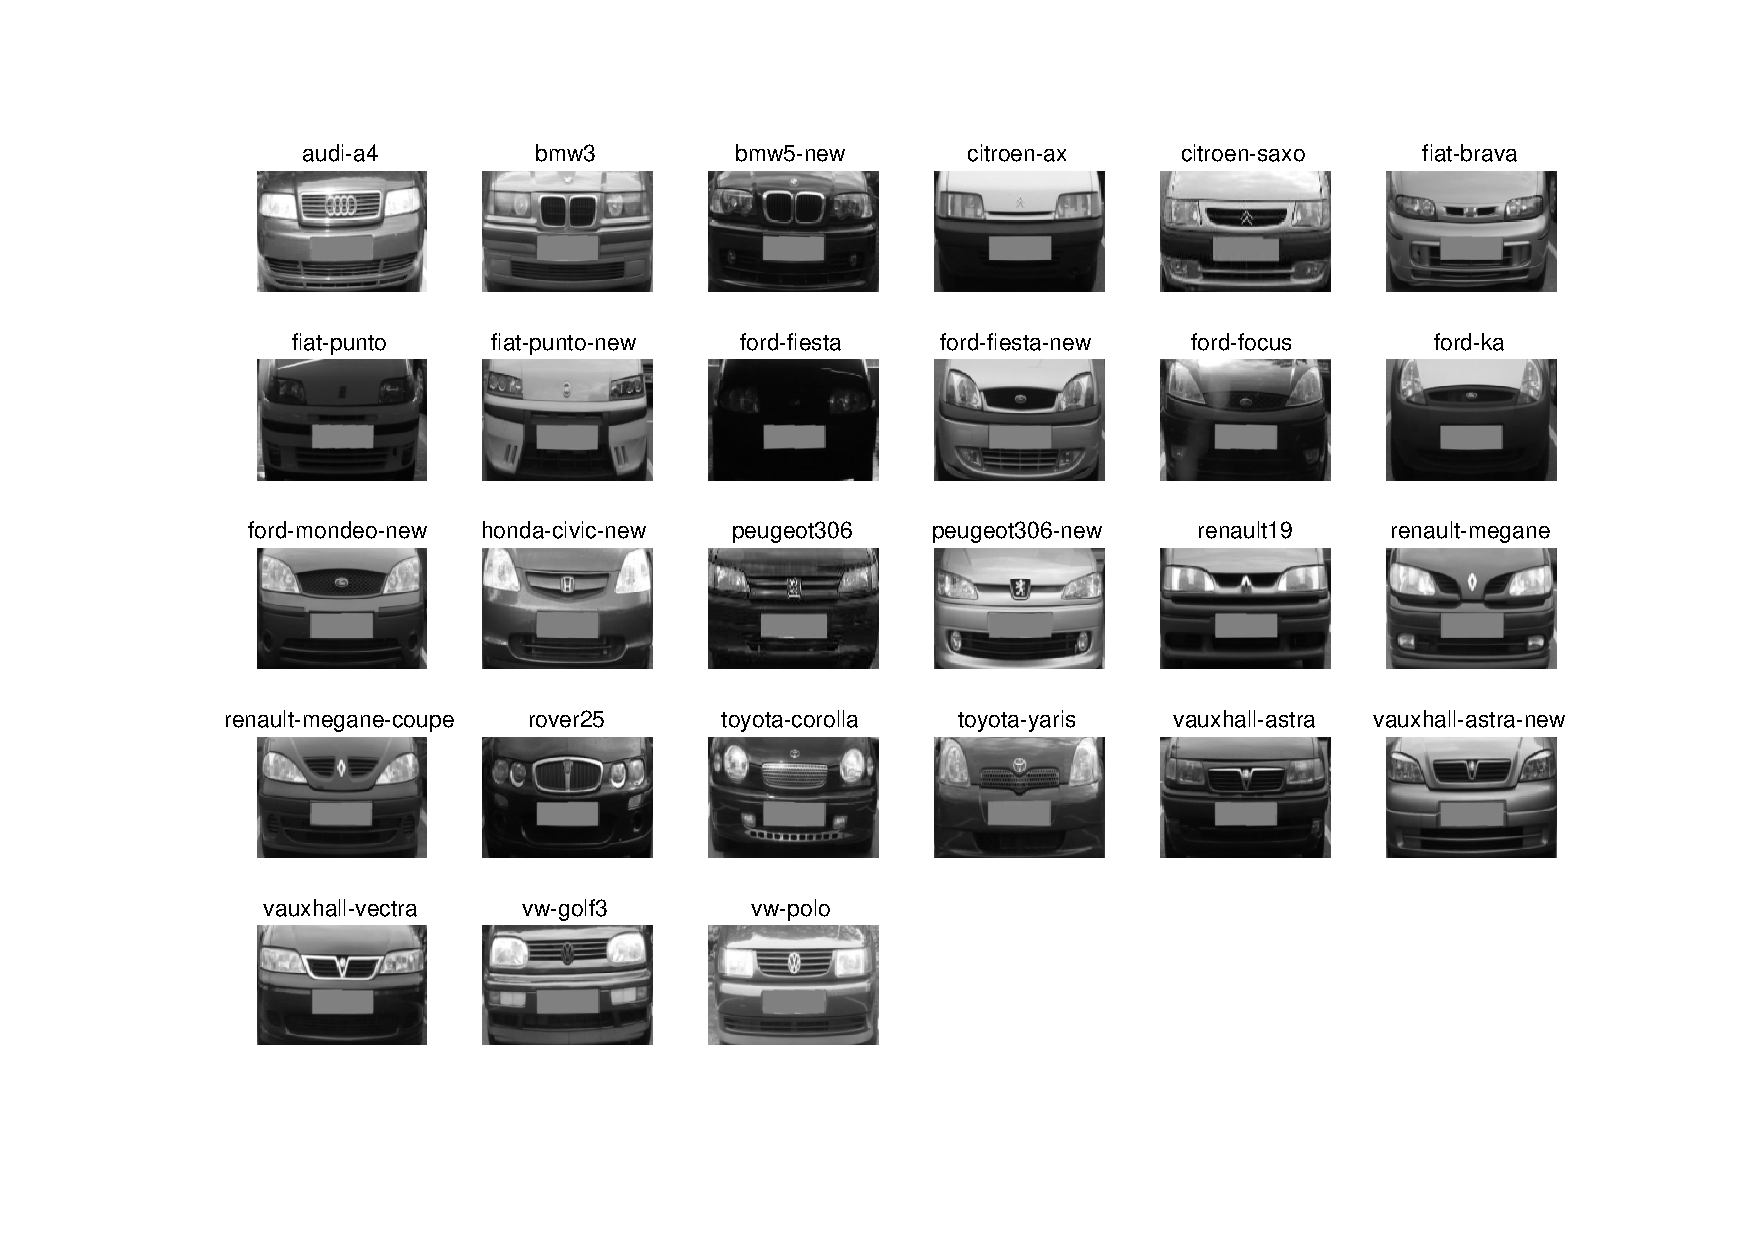
\includegraphics{classes}
\caption{Samples of All $27$ Vehicle Make and Model Classes in the Dataset.}
\label{fig:classes}
\end{figure}

\section{Comparison to Our Method}

In this paper, we make use of 
Raw Image Pixels, Sobel Edge Response and Square Mapped Gradients following Petrovic and Cootes's \citep{petrovic2004analysis} work, 
Locally Normalised Harris Strengths (LNHS) from Pearce and Pears's work \citep{pearce2011automatic}, and 
Bag of Speeded Up Robust Features (SURF) from Siddiqui et al.'s work \citep{siddiqui2016real} 
interchangeably in our features extraction module.
We use Principal Component Analysis (PCA) for optional dimensionality reduction module and either 
K-Nearest Neighbour (KNN) or
Support Vector Machine (SVM) for classification module.

Despite the simplicity of features computation compared to Mid-Level-Representation in Fraz et al.'s work \citep{fraz2014mid}, our method achieves a higher accuracy score of $99\%$ on the dataset.






